\documentclass[dvipdfmx]{standalone}
\usepackage{tikz}
\usepackage[latin1]{inputenc}
\usetikzlibrary{shapes,arrows,shapes,shapes.geometric,calc}
\usetikzlibrary{positioning}


\begin{document}
\begin{tikzpicture}[scale=1]
    \tikzset{frame/.style={rectangle, draw, text width=1.8cm, text centered, minimum height=2.4cm, }};
    \tikzset{empty/.style={rectangle}};
    \node[empty](em) at (0cm,7.5cm){};
    \node[empty](em) at (12.5cm,1.2cm){};

    \node [frame](lapa) at (6cm, 6.1cm){};
    \node [frame](lapb) at (6cm, 2.6cm){};

    \node (user) at (1cm, 4.35cm)[scale=0.2] {
\includegraphics{../attack-model/image/smart.png}};
    \node (lap1) at (6cm, 6.5cm) [scale=0.15] {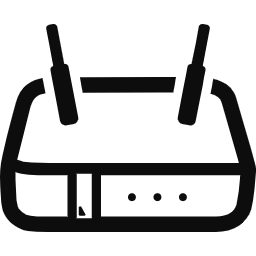
\includegraphics{../attack-model/image/lap.png}};
    \draw [very thick] (7cm,6.1cm)--(10.7cm,4.35cm);
    \draw[very thick,densely dashed,->] (1.5cm, 4.35cm) -- (5.3cm, 5.55cm);
    \node (lap2) at (6cm, 3cm) [scale=0.15] {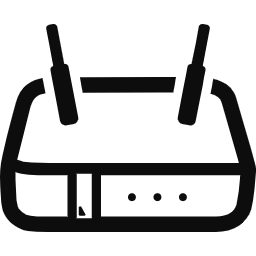
\includegraphics{../attack-model/image/lap.png}};
    \draw [very thick] (7cm,2.6cm)--(10.7cm,4.35cm);
    \node (gateway) at (11cm, 4.35cm) {
\includegraphics[scale=0.2]{../attack-model/image/gateway.png}};
    \draw (5.4cm,5.55cm) circle [radius=1.5pt];
    \fill (5.4cm,5.55cm) circle [radius=1.5pt];
    \draw (5.4cm,5.15cm) circle [radius=1.5pt];
    \fill (5.4cm,5.15cm) circle [radius=1.5pt];
    \draw (5.4cm,2.05cm) circle [radius=1.5pt];
    \fill (5.4cm,2.05cm) circle [radius=1.5pt];
    \draw (5.4cm,1.65cm) circle [radius=1.5pt];
    \fill (5.4cm,1.65cm) circle [radius=1.5pt];
    \coordinate(return) at (6cm, 5.8cm) node at (return)  [below] {\Large $m_A$};
    \coordinate(return) at (6cm, 5.4cm) node at (return)  [below] {\Large $m_a$};
    \coordinate(return) at (6.1cm, 4.9cm) node at (return)  [below] {\Large $\rm LAP (a)$};

    \coordinate(return) at (6cm, 2.3cm) node at (return)  [below] {\Large $m_B$};
    \coordinate(return) at (6cm, 1.9cm) node at (return)  [below] {\Large $m_b$};
    \coordinate(return) at (6.1cm, 1.4cm) node at (return)  [below] {\Large $\rm LAP (b)$};
    \coordinate(return) at (1cm, 3.4cm) node at (return)  [below] {\Large $\rm User\ Device$};
    \coordinate(return) at (11cm, 3.4cm) node at (return)  [below] {\Large $\rm Gateway$};

\end{tikzpicture}
\end{document}documentclass{standalone}
\usepackage{tikz}
\usepackage[latin1]{inputenc}
\usetikzlibrary{shapes,arrows,shapes,shapes.geometric,shadows}
\usetikzlibrary{positioning}
\begin{document}
\begin{tikzpicture}[]
\end{tikzpicture}
\end{document}
